\documentclass{article}

\usepackage[total={6in, 8in}]{geometry}
\usepackage[utf8]{inputenc}
\usepackage[english]{babel}
\usepackage{lipsum}  

\usepackage{float}
\usepackage{amsmath}
\usepackage{amssymb}
\usepackage{apacite}
\usepackage{siunitx}
\usepackage{graphicx}
\graphicspath{ {images/} }
\usepackage{pgfplots}
\usepackage{pgfplotstable}
\usepackage{pgfkeys}

\pgfkeys{
  /pgf/number format/textnumber/.style={
    precision=4,
  },
}

\newcommand{\pError}[0]{\ensuremath{\% \text{Error}}}
\newcommand{\foundGrating}[0]{\ensuremath{\num{1.87e-6} \: \si{m}}}
\newcommand{\givenGrating}[0]{\ensuremath{\num{1.90e-6} \: \si{m}}}
\newcommand{\length}[0]{\ensuremath{\num{255} \: \si{cm}}}
\newcommand{\twocol}[2]{\multicolumn{2}{|cc|}{#1 & #2}}

\title{Balmer Series}
\author{Kyle McKean \\ \normalsize Mattie O'Kelley}
\date{\normalsize FLO1 Box 22}

\begin{document}
\maketitle
\begin{abstract}
\lipsum[1-1]
\end{abstract}
\section{Introduction}
\begin{equation}
  \pError = \left| \frac{O - E}{E} \right| \cdot 100
\end{equation}
In the following tables percent error is calculated with the above equation. 
\begin{equation}
  \label{eq:dist}
  \sin{\theta} = \frac{x}{\sqrt{L^2 + x^2}}
\end{equation}
\begin{equation}
  \label{eq:relation}
  d \sin{\theta} = m \lambda
\end{equation}
\begin{equation}
  \label{eq:rydberg-1}
  R = - \frac{Z^2e^4m_e}{8\epsilon_0^2n^2h^2}
\end{equation}
\begin{equation}
  \label{eq:rydberg-2}
  \frac{1}{\lambda} = R_H \left( \frac{1}{n_f^2} - \frac{1}{n_i^2} \right)
\end{equation}
$R_H$ is $R$ using $n = 1$ and $Z = 1$.
\begin{equation}
  \label{eq:rydberg-3}
  \frac{1}{\lambda} = R_H \left( \frac{1}{2^2} - \frac{1}{n_i^2} \right)
\end{equation}

\section{Experimental Design and Procedure}
\lipsum[5-6]
\section{Results and Analysis}
\subsection{Part One}
The length $(L)$ from the laser to the wall was $0.808 \: \si{m}$.
The wavelength $(\lambda)$ of the laser was $650 \: \si{nm}$.
The average distance between the maximum was $0.2985 \: \si{m}$.
Using these facts and the above equations (\ref{eq:dist}, \ref{eq:relation})
we learn $d$ is equal to $\foundGrating$. This is $1.57\%$ off the expected
$d = \givenGrating$.
\subsection{Part Two}

The observed wavelength calculations appear in the appendix in Table (\ref{table:hydrogen-distances}).
The expected wavelengths are found in Table 1 of (CITEME).
\begin{table}[h!]
  \centering
  \begin{tabular}{ |cc|c|c|c| }
    \hline
    $n_i$ & Color & Expected Wavelength $(\si{m})$ & Observed Wavelength $(\si{nm})$ & $\pError$ \\
    \hline
    $3$ & (Red)    & $656$ & $641$ & $2.28$ \\
    $4$ & (Blue)   & $486$ & $469$ & $3.50$ \\
    $5$ & (Violet) & $434$ & $411$ & $5.30$ \\
    \hline
  \end{tabular}
  \caption{
    Hydrogen spectral lines
  }
\end{table}

\begin{figure}[H]
  \centering
  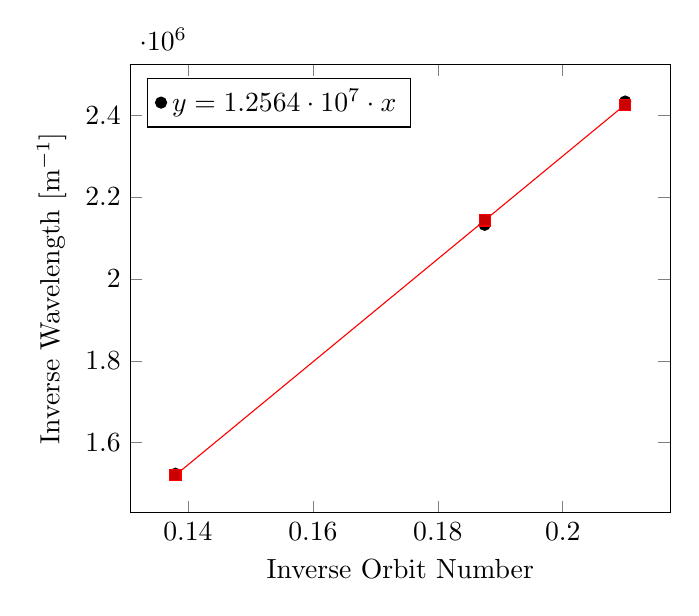
\begin{tikzpicture}
      % \pgfplotsset{width=10cm,
          % compat=1.3,
          % legend style={font=\footnotesize}}
      \begin{axis}[
      xlabel={Inverse Orbit Number},
      ylabel={Inverse Wavelength $[\si{m^{-1}}]$},
      legend cell align=left,
      legend pos=north west]
      \addplot[only marks] table[row sep=\\]{
          X Y\\
          0.138  1524390\\
          0.1875 2132196\\
          0.21   2433090\\
      };
      \addplot table[row sep=\\,
      y={create col/linear regression={y=Y}}]
      {
          X Y\\
          0.138  1524390\\
          0.1875 2132196\\
          0.21   2433090\\
      };
      \addlegendentry{$y = \pgfmathprintnumber[textnumber]{\pgfplotstableregressiona} \cdot x$}
      \end{axis}
  \end{tikzpicture}
\end{figure}

The observed wavelength calculations appear in the appendix in Table (\ref{table:hydrogen-distances}).
The expected wavelengths are found in Table 1 of (CITEME).
\begin{table}[h!]
  \centering
  \begin{tabular}{ |cc|c|c|c| }
    \hline
    $n_i$ & Color & Expected Wavelength $(\si{m})$ & Observed Wavelength $(\si{nm})$ & $\pError$ \\
    \hline
    $3$ & (Red)    & $687$ & $654$ & $4.80$ \\
    $4$ & (Orange) & $588$ & $578$ & $1.70$ \\
    $5$ & (Green)  & $471$ & $492$ & $4.46$ \\
    $6$ & (Blue)   & $438$ & $435$ & $0.68$ \\
    \hline
  \end{tabular}
  \caption{
    Helium spectral lines
  }
\end{table}

\begin{figure}[H]
  \centering
  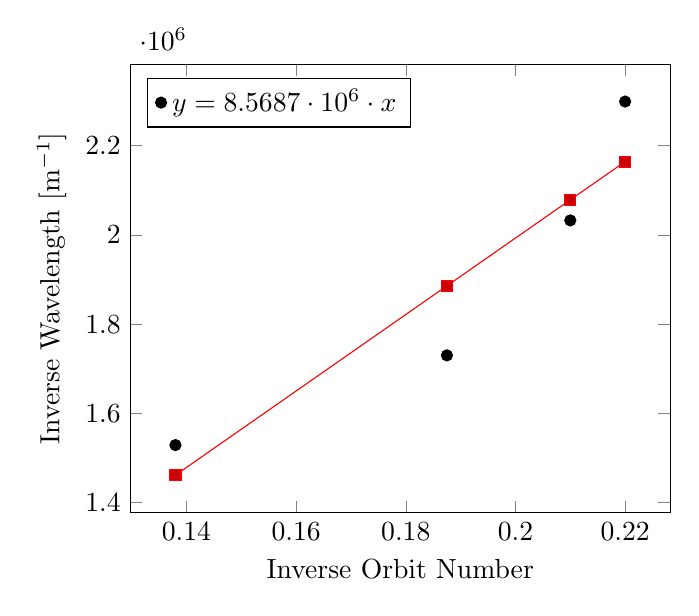
\begin{tikzpicture}
      % \pgfplotsset{width=10cm,
          % compat=1.3,
          % legend style={font=\footnotesize}}
      \begin{axis}[
      xlabel={Inverse Orbit Number},
      ylabel={Inverse Wavelength $[\si{m^{-1}}]$},
      legend cell align=left,
      legend pos=north west]
      \addplot[only marks] table[row sep=\\]{
          X Y\\
          0.138  1529051\\
          0.1875 1730103\\
          0.21   2032520\\
          0.22   2298850\\
      };
      \addplot table[row sep=\\,
      y={create col/linear regression={y=Y}}]
      {
          X Y\\
          0.138  1529051\\
          0.1875 1730103\\
          0.21   2032520\\
          0.22   2298850\\
      };
      \addlegendentry{$y = \pgfmathprintnumber[textnumber]{\pgfplotstableregressiona} \cdot x$}
      \end{axis}
  \end{tikzpicture}
\end{figure}

The expected Rydberg constant for Helium is $R_{He} = \num{4.36e-7} \: \si{m^{-1}}$.
The line of best fit is off by $1868\%$.

\section{Conclusions}

\lipsum[8-9]

\section{Appendix}

The observed wavelength was calculated using equations (\ref{eq:dist},
\ref{eq:relation}) where $d = \givenGrating$ and $L = \length$.

\begin{table}[h!]
  \centering
  \begin{tabular}{ |c|c|c| }
    \hline
    Observed Color & Average Distance from Maximum $(\si{cm})$ & Wavelength $(\si{nm})$ \\
    \hline
    Red    & $91.5$ & $641$ \\
    Blue   & $65.0$ & $469$ \\
    Violet & $56.5$ & $411$ \\
    \hline
  \end{tabular}
  \caption{
    Hydrogen spectral lines
  }
  \label{table:hydrogen-distances}
\end{table}

\begin{table}[h!]
  \centering
  \begin{tabular}{ |c|c|c| }
    \hline
    Observed Color & Average Distance from Maximum $(\si{cm})$ & Wavelength $(\si{nm})$ \\
    \hline
    Red    & $93.5$ & $654$ \\
    Orange & $81.5$ & $578$ \\
    Green  & $68.5$ & $492$ \\
    Blue   & $60.0$ & $435$ \\
    \hline
  \end{tabular}
  \caption{
    Helium spectral lines
  }
  \label{table:helium-distances}
\end{table}


\bibliographystyle{apacite}
\bibliography{citation.bib}
\end{document}